\chapter{Zabezpečení a autentizace}
V této kapitole si projdeme základní autentizační protokoly a standardy, pro jednoduchost se zaměříme na standardy OpenAPI ve verzi 3.0. Autorizace se v našem případě používá především pro prevenci zneužití a kontrolu nad tím, kdo API používá a jak často se k němu přistupuje.


\section{API key}
%odkaz na api key zdroj https://swagger.io/docs/specification/authentication/api-keys/
% https://www.fortinet.com/resources/cyberglossary/api-key#:~:text=API%20Keys%20Definition%20and%20Meaning,a%20white%2Dlabeled%20internal%20marketplace.
API klíč je unikátní token, který umožňuje uživateli se autorizovat, a následně dostat oprávnění, na která má nárok. Klíč může být poslán jako query param \texttt{GET /users?key=rea11ysecr5tApIKeY}, v hlavičce requestu či jako Cookie \texttt{X-KEY: rea11ysecr5tApIKeY}. API klíč by měl znát jen server a daný klient, proto je autentizace brána jako bezpečná pouze při použití dalších bezpečnostních prvků jako je třeba HTTPS/SSL.

\subsection{Popis API klíče}
\begin{listing}[ht]
    \inputminted[]{yaml}{resources/code/security/openapi-key.yml}
    \caption{Definice OpenAPI 3.0}
    \label{code:api_key}
\end{listing}

Nejčastější použití API klíče je pro blokování anonymních požadavků, pomocí čehož je možné vyfiltrovat případný škodlivý provoz na API. Díky jeho jednoduchosti se také často používá mezi IoT zařízeními.

V tomto příkladě je definován název API key (\texttt{X-API-key}), který bude přenesen v headeru (Výpis \ref{code:api_key}, řádek 8). Dále s ním můžeme pracovat jako s \texttt{ApiKeyAuth} a dávat jej do všech ostatních definicí endpointů, pokud by bylo třeba specifikovat (Výpis \ref{code:api_key}, řádek 20, 21). Pokud potřeba není (Výpis \ref{code:api_key}, řádek 11, 12), autorizaci aplikujeme na všechny operace.

API klíčů může být využito víc, například pro specifikování uživatele nebo aplikace.

Při nevalidním nebo chybějícím klíči můžeme vrátit chybový kód 401, který značí neoprávněný přístup (Výpis \ref{code:api_key} řádek 11-16).


\section{Json Web Token} %TODO cite or smthng https://jwt.io/introduction
\label{sec:jwt}
JWT je otevřená industriální standardizovaná % \verb|\glossary{rfc7519}| TODO
metoda pro bezpečné přeposílání zpráv ve formátu JSON mezi dvěma stranami. Tyto objekty mohou být zkontrolovány a následně je možné ověřit jejich autenticitu, protože jsou digitálně podepsány prostřednictvím tajného klíče nebo páru veřejného a privátního klíče za pomocí RSA nebo ECDSA algoritmu.

Nejčastěji se používá pro \textbf{autorizaci} a pro \textbf{výměnu informací}. Při autorizaci se uživatel jednou přihlásí a každý jeho další požadavek bude s JWT, což mu dovoluje přistupovat i tam, kde by bez přihlášení nemohl. Single Sign On %\verb|\ref{sso} (btw všb přihlašováky)| TODO
využívá JWT především díky malé režii a jednoduchosti použití v různých doménách. JSON web tokeny jsou taktéž dobrý způsob jak bezpečně \textbf{vyměňovat informace} mezi více stranami díky digitálním podpisům.

\subsection{Struktura}
V kompaktní zakódované formě JWT vypadá takto: \texttt{xxxxxx.yyyyyyy.zzzzzz}. V tomto formátu je \texttt{x} je zakódovaný header, \texttt{y} je payload a \texttt{z} je podpis.

\begin{description}
    \item[Header] Typicky se skládá ze dvou částí -- typ tokenu a podepisovací algoritmus který byl použit, například SHA256 nebo RSA. (Výpis \ref{code:JWT_example}, řádek 3)
    \item[Payload] Obsahuje data o entitě a jiné informace. (Výpis \ref{code:JWT_example} řádek 9)
    \item[Signature] Podpis se vytvoří kombinací headeru, payloadu a secretu a zašifruje se příslušným algoritmem. (Výpis \ref{code:JWT_example}, řádek 15)
\end{description}

\begin{listing}[ht]
    \inputminted[]{json}{resources/code/security/JWT.jsonc}
    \caption{Příklad hlavičky, obsahu a podpisu v JWT} % TODO whatever nějaké cite nebo něco https://jwt.io/introduction
    \label{code:JWT_example}
\end{listing}


\section{OAuth 2.0}
OAuth 2.0 je autorizační framework, který poskytuje limitovaný přístup k datům. Nahrazuje OAuth z roku 2012 a dnes se již považuje za standard pro online autorizaci. Poskytuje přístup a omezuje akce, které s day může klientská aplikace provádět, bez toho, aby bylo třeba sdílet přihlašovací údaje uživatele.
% TODO kdyžtak jak to vypadá ve švagrovi


\subsection{Principy}
Jedná se o autorizační, nikoli autentizační protokol, což znamená, že je určen pro získání přístupových práv ke zdrojům, ne k ověření identity uživatele, i když v praxi se často používá pro oba účely.

Používají se zde přístupové tokeny, které jsou reprezentovány řetězcem a poskytují oprávnění k přístupu k datům. I přesto, že Oauth 2.0 nemá nijak definovaný formát přístupového tokenu, nejčastěji se využívá JWT (TODO glossary json web token). Tokeny mohou mít také datum vypršení platnosti, což znamená, že po uplynutí tohoto data je třeba získat nový token.


\subsection{Role}\label{sec:Oauth_roles}
V této části se zaměříme na klíčové role v procesu autentizace a autorizace v rámci OAuth 2.0 protokolu.

\begin{description}
    \item[Resource owner] je uživatel, který povoluje přístup aplikace k jeho účtu, jenž je limitován rozsahem uděleného oprávnění.
    \item[Client] je aplikace, která žádá o přístup k uživatelskému účtu. Tu musí nejdříve uživatel oprávnit a oprávnění musí validováno API.
    \item[Resource server] má uložená uživatelská data a HTTP služby,které mohou poskytovat uživatelská data autentizovaným klientům.
    \item[Authorization server] je zodpovědný za ověření uživatelské identity a poskytování autentizačního tokenu. Tento token je následně přijímán resource serverem.
\end{description}


\begin{figure}[H]
    \centering
    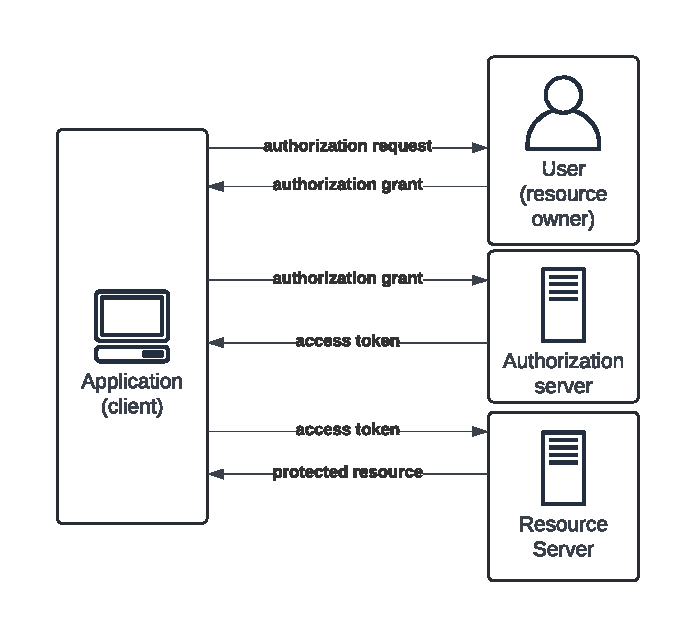
\includegraphics[width=\textwidth]{figures/OAuth_abstract_flow.pdf}
    \caption{Abstraktní průběh protokolu}%\cite{https://medium.com/@greekykhs/ro-acd8cb4cc0f4#:~:text=OAuth%202.0%20defines%20four%20roles,Resource%20Server%20and%20Authorization%20Server.}} TODO 
    \label{fig:Oauth_roles_diagram}
\end{figure}


\subsection{Grant type: Authorization code}
Jedná se o nejčastěji používanou metodu, především z důvodu optimalizace pro stranu serveru. Autorizační server zde vrací autorizační kód na jedno použití, který je pak vyměněn za přístupový token, podobně jako když se uživatelé přihlašují do webových aplikací s jejich Facebook nebo Google účtem.

\begin{figure}[ht]
    \centering
    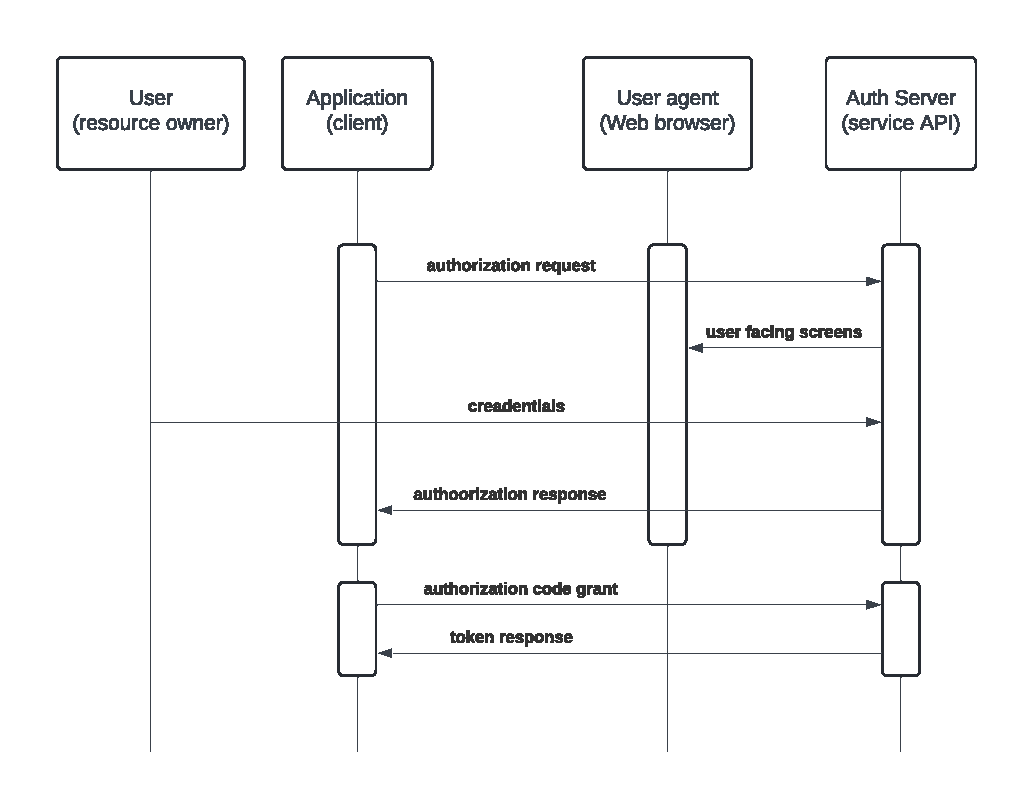
\includegraphics[width=\textwidth]{figures/Oauth auth flow.pdf}
    \caption[short]{Průběh autorizace pomocí autorizačního kódu}%TODO https://www.digitalocean.com/community/tutorials/an-introduction-to-oauth-2
    \label{fig:Oauth_auth_flow}
\end{figure}


Na obrázku \ref{fig:Oauth_auth_flow} je popsán průběh výměny autorizačního kódu.
Jedná se o dvoufázový proces.
Nejdříve je aplikace vytvoří autorizační URL a otevře ji v prohlížeči, zde se uživatel přihlásí a tím se ověří na autorizačním serveru, takže aplikace nebude mít informace o uživatelských přihlašovacích údajích. Aplikace poté v odpovědi obdrží autorizační kód a ten je poté odeslán zpět na autorizační server, který vrátí přístupový token.


\section{Shrnutí}
Jako nejvhodnější styl zabezpečení pro modelovou hru se zdá být API klíč, a to z důvodu jeho jednoduchosti na implementaci, i přes to, že v případě, kdy se uživatelé přihlašují, je vhodný také OAuth2. Z časových důvodů a kvůli nízké škále uživatelských privilegií (administátor, který bude používat backoffice s přímým přístupem na databázi, a uživatelé, kteří budou hru hrát) jsme vybrali právě API klíč.

